\documentclass[11pt]{article} %article 文档
 \usepackage{color}
\usepackage{amsmath}
\usepackage{setspace}
\usepackage{graphicx}
\usepackage{caption}
\usepackage{hyperref}
\hypersetup{hidelinks,
	colorlinks=true,
	allcolors=black,
	pdfstartview=Fit,
	breaklinks=true}
\captionsetup[figure]{labelfont=bf, name=Figure, labelsep=period}
\newcommand{\reffig}[1]{Fig.\ref{#1}}
\setstretch{1.523} 
\title{COMP90007 Assignment 1}  %文章标题
\author{Student Name : Handan Yu\\ Student ID : 1235484}
\usepackage[a4paper,left=10mm,right=10mm,top=15mm,bottom=15mm]{geometry}  
\usepackage{enumerate}
\newtheorem{Q}{Ans}
\begin{document}
\date{}
\maketitle 
 \begin{Q}
 \end{Q}
Compared with OSI, using a 5-layer hybrid network reference model is much more simple, cost-effective, accessible and high-efficiency. Also, unlike TCP/IP model, the concepts of services, interfaces and protocols can be clearly distinguished by using a 5-layer hybrid network reference model.\\
 \begin{Q}
 \end{Q}
 \begin{enumerate}[(1)]
 \item T-delay = $\frac{5\times 1280\times 720\text{pixels} \times3\text{bytes/pixel}}{256\text{kbps}} =432 \text{ seconds}$, 
 P-delay = $\frac{1500\text{km}}{200000\text{km/s}} = 7.5\times 10^{-3}\text{ seconds}$,\\
 Latency = T-delay + P-delay = 432.0075 seconds.
 \item T-delay = $\frac{5\times 1280\times 720\text{pixels} \times3\text{bytes/pixel}}{1\text{Gbps}} =0.110592 \text{ seconds}$,
 P-delay = $ \frac{1500\text{km}}{200000\text{km/s}} = 7.5\times 10^{-3}\text{ seconds} $,\\
 Latency = T-delay + P-delay = 0.1180092 seconds.\\
  \end{enumerate}
  \begin{Q}
 \end{Q}
Nyquist’s limit:  Max. data rate = $2\times 16\text{k}\log_28\text{ bits/sec} = 96 \text{ kbps}$,\\
Shannon’s limit: Max. data rate = $16\text{k}\times \log_2(1+100) \text{bits/sec} \approx 106.53 \text{ kbps}$,\\
 Since, $96 \text{ kbps} < 106.53 \text{ kbps}$, the max data rate of this channel is 96 kbps.\\
  \begin{Q}
 \end{Q}
 Since the number of data is 4, the number of check bits is 3.
 Then we can assume the data sent is like
 \begin{center}
 \begin{tabular}{|c|c|c|c|c|c|c|}
 \hline
 P1&P2&P3&P4&P5&P6&P7\\
 \hline
 ?&?&1&?&0&0&0\\
 \hline
 \end{tabular}
 \end{center}
Next, calculate the parity bits for P1, P2, P4.
\begin{center}
P1 + P3 + P5 + P7 = ?+1+0+0 (odd)  P1 = 0\\
P2 + P3 + P6 + P7 = ?+1+0+0 (odd)   P2 = 0\\
P4 + P5 + P6 + P7 = ?+0+0+0 (even) P4 = 1\\
 \end{center}
 Therefore, the data 0011000 will be  transmitted.
 \\
  \begin{Q}
 \end{Q}
 
 Firstly, I chose the certain traffic to monitor and set the 'tcp port http' as the capture filter. Then I ticked 'resolve network names' and unticked 'enable promiscuous mode on all interfaces'.  After starting capture, I opened the website \href{http://archive.ics.uci.edu/ml/index.php}{http://archive.ics.uci.edu/ml/index.php}
  
\reffig{connect} shows the CONNECT primitive. Since three-way handshake can be seen as a way of how TCP connection is established,  the red frame part of \reffig{connect} is the three-way handshake process. Also, after these three steps, HTTP protocol sent info 'GET' to the client.

\reffig{send} shows the process of sending data. As we can see from the part marked in blue, the HTTP protocol sent info 'OK' to the client, which means it had received the data(i.e. image) sent from the client. Therefore, the TCP streams above that (i.e. the part framed in red) is the SEND primitive.

  \begin{figure}[htbp]
 \centering
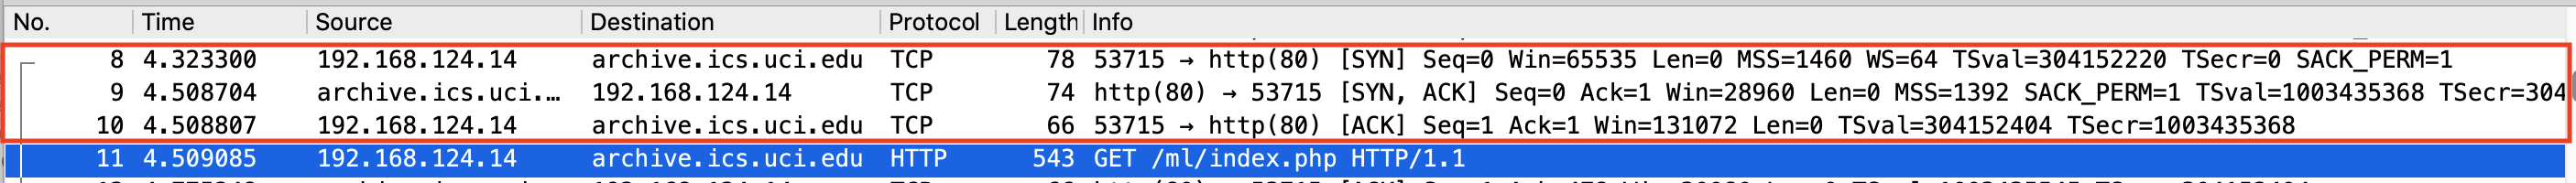
\includegraphics[height=1.7cm,width=19cm]{img/connect.png}
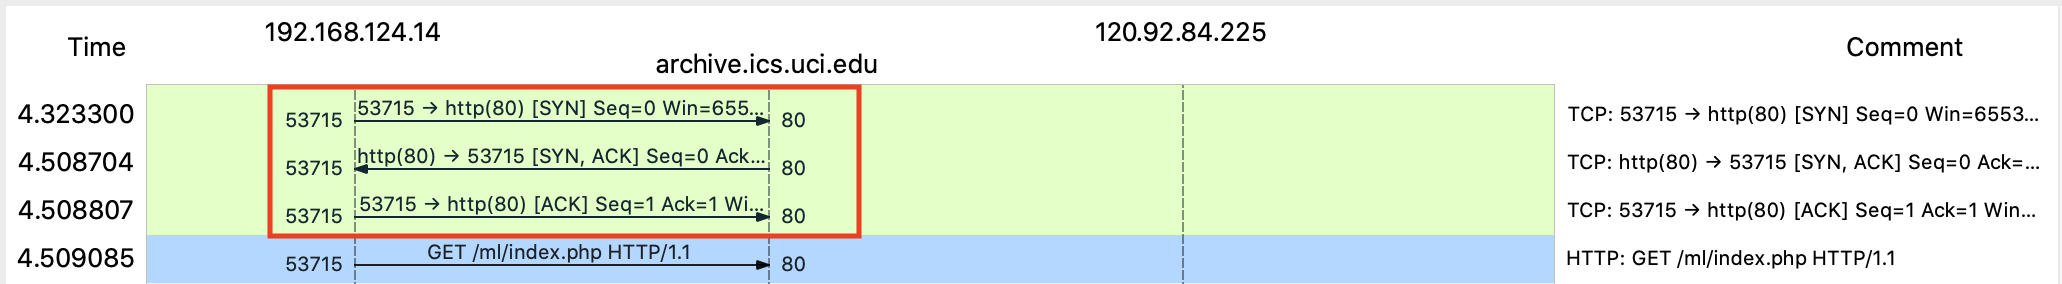
\includegraphics[height=1.7cm,width=13cm]{img/CONNECT_1.png}
\caption{CONNECT}\label{connect}
 \end{figure}
   \begin{figure}[htbp]
 \centering
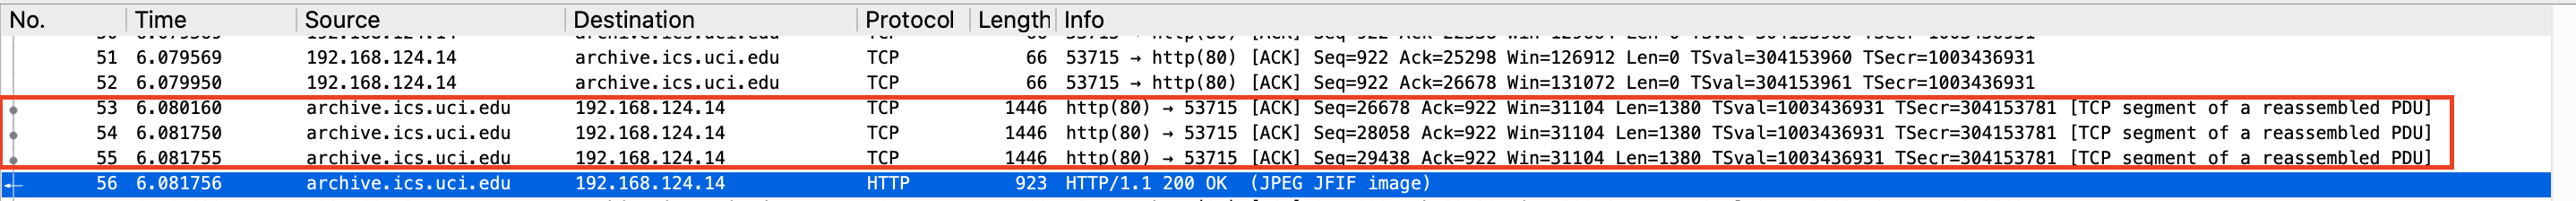
\includegraphics[height=1.4cm,width=19cm]{img/send.png}
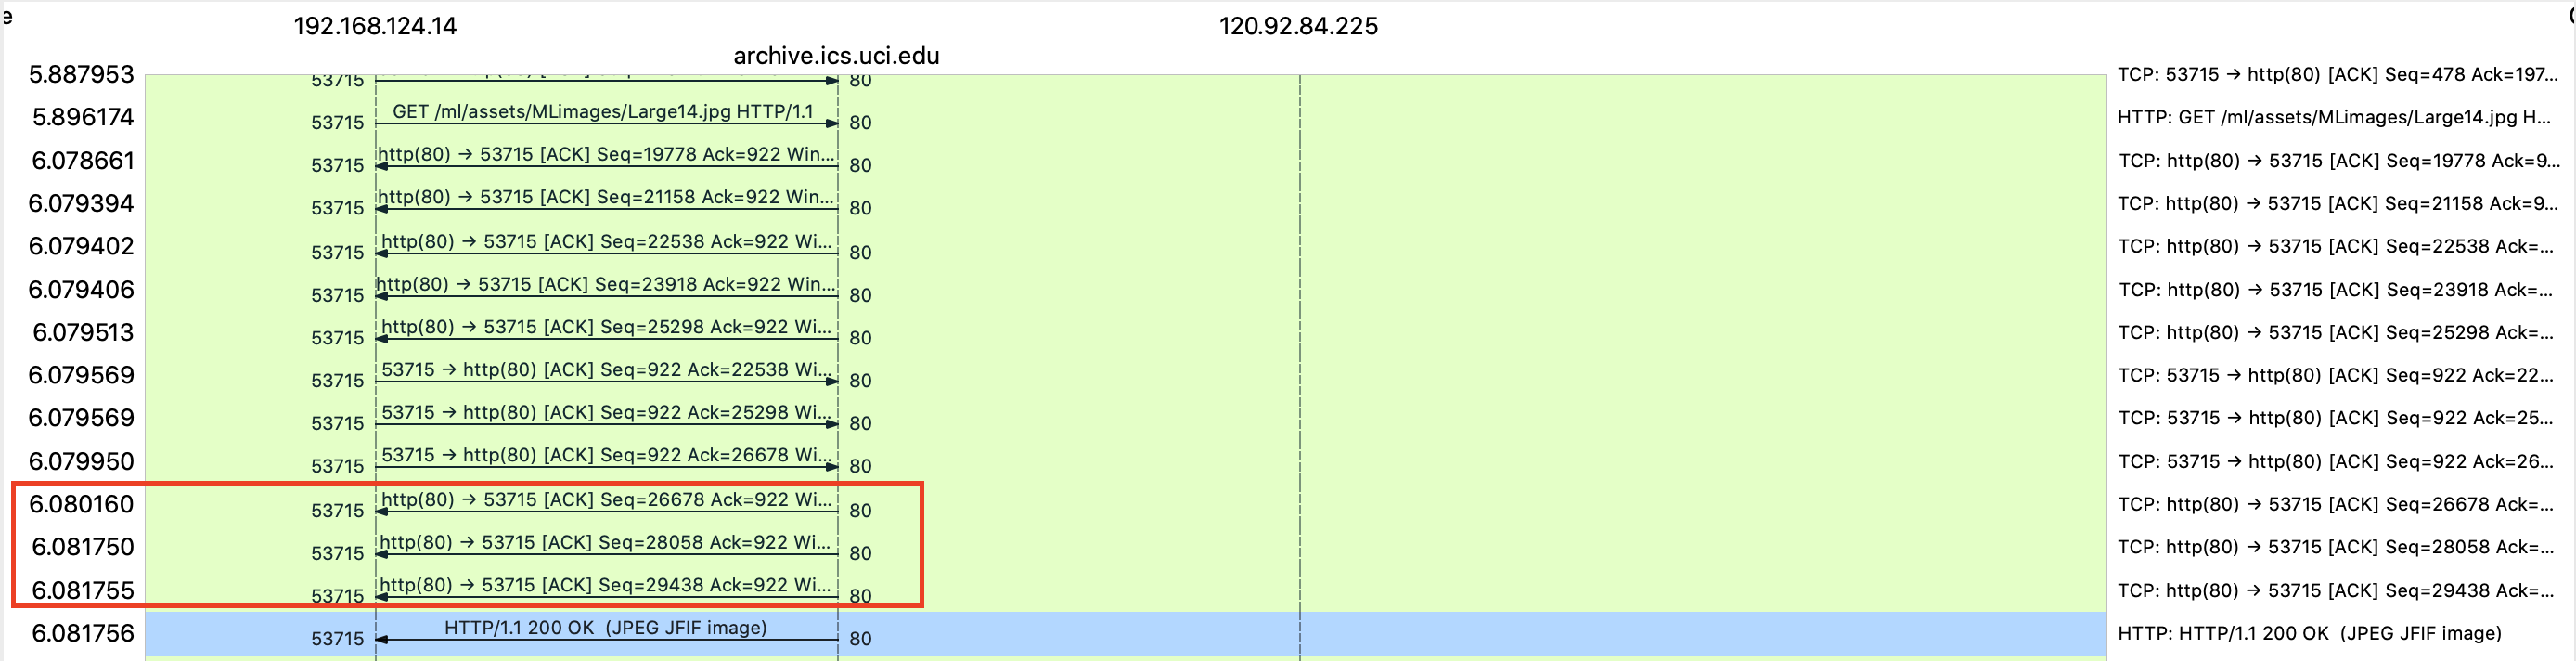
\includegraphics[height=3cm,width=13cm]{img/SEND_1.png}
\caption{SEND}\label{send}
 \end{figure}
\end{document}